\section{\esp Problema de Escalonamento e Roteamento de Enfermeiras }\label{pad}

Nesta seção será apresentado a definição do \acl{PERE} e as métricas utilizadas por cada autor para solucionar suas variações.
%Entre as diversas variações do \ac{PERE}, foi encontrado no artigo de \citeonline{tricoire:2016} uma definição que descreve o \ac{PERE} de forma genérica.
Segundo \citeonline{tricoire:2016}, dado o conjunto $E$ de enfermeiras e o conjunto $S$ de serviços solicitados por um ou mais pacientes $p \in P$. 
O \ac{PERE} tem como objetivo encontrar uma rota para cada veículo e um escalonamento para cada enfermeira do \ac{SAD}, indicando quais tarefas devem ser cumpridas por cada enfermeira, em qual ordem e em qual momento, de forma a não ultrapassar a carga horária máxima prevista em lei.

Cada paciente $p\in P$ pode requisitar um ou mais serviços $s \in S$ que serão executados pela enfermeira $e \in E$  que possui a qualificação necessária para executar determinado serviço $s \in S$ com a duração de tempo necessária para que o serviço seja completo. O limite superior e inferior para o início do serviço é definido por uma janela de tempo $[e_i, l_i]$.

Além de considerar os locais e os pacientes a partir da mesma variável, \citeonline{Bierwirth:2013} considerou em seu trabalho as enfermeiras e os veículos a partir da utilização da mesma variável, uma vez que existe um veículo para cada enfermeira, ou para cada conjunto de enfermeiras que possuem a mesma qualificação.

As rotas do \ac{PERE} podem ser modeladas a partir de um grafo  $G = (V, A)$ no qual $V= \{ v_0, v_1, \ldots, v_{|V|} \}$ é um conjunto de vértices, tal que o vértice $v_0$ representa o local de partida e de chegada das enfermeiras e os demais representam os locais de atendimento. O conjunto de arestas $A = \{(i,j): i\in V, j \in V, i \neq j\}$ representa o translado entre dois locais. 
Cada aresta possui um custo associado $c_{ij}$, representando o tempo de translado entre os locais $v_i$ e $v_j$.
Na Figura \ref{grafo1}, é apresentado o exemplo de uma instância, contendo três rotas, sendo cada rota representa o caminho percorrido por uma enfermeira, que parte do hospital, atende a um conjunto de pacientes e retorna ao hospital.

Uma parte da solução para o \ac{PERE} pode ser representada a partir de uma matriz $M_{|P|\times |S|}$, na qual cada célula $m_{p_i,s_j} \in M$ contém a atribuição de cada paciente a um ou mais serviços previamente requisitados, como pode ser visto na Tabela \ref{paciente_serviço}.
E de uma matriz $M_{|E|\times |S|}$, na qual cada célula $m_{e_i,s_j} \in M$ contém a atribuição de cada enfermeira ao serviço ao qual está apta a executar, como pode ser visto na Tabela \ref{enfermeira_serviço}.

Cada atribuição é definida a partir dos valores $0$ e $1$, sendo o valor $1$ representa que o paciente requisitou o serviço ou que a enfermeira está apta para realizar determinado serviço e $0$ caso contrário. \\

\begin{table}[!ht]
\centering
\caption{Exemplo da atribuição de pacientes a serviços \label{paciente_serviço}}
\begin{tabular}{c|c|l|l|l|l|l}
   & s1 & s2 & s3 & s4 & s5 & s6 \\ \hline
p1 & 1  & 0  & 0  & 1  & 0  & 0  \\ \hline
p2 & 0  & 1  & 1  & 0  & 0  & 0  \\ \hline
p3 & 1  & 0  & 1  & 0  & 1  & 0  \\ \hline
p4 & 0  & 0  & 0  & 0  & 0  & 1  \\ \hline
\end{tabular}
{\footnotesize\\ \textbf{Fonte: Autoria Própria (2018)}}
\end{table}


\begin{table}[!ht]
\centering
\caption{Exemplo da atribuição de enfermeiras a serviços \label{enfermeira_serviço}}
\begin{tabular}{c|c|l|l|l|l|l}
   & s1 & s2 & s3 & s4 & s5 & s6\\ \hline
e1 & 0  & 0  & 0  & 1  & 0  & 0  \\ \hline
e2 & 0  & 0  & 0  & 0  & 0  & 1  \\ \hline
e3 & 1  & 0  & 0  & 0  & 0  & 0  \\ \hline
e4 & 0  & 1  & 0  & 0  & 0  & 0  \\ \hline
e5 & 0  & 0  & 0  & 0  & 1  & 0  \\ \hline
e6 & 0  & 0  & 1  & 0  & 0  & 0  \\ \hline
\end{tabular}
{\footnotesize\\ \textbf{Fonte: Autoria Própria (2018)}}
\end{table}




\begin{figure}[!ht]
\centering
\begin{center}
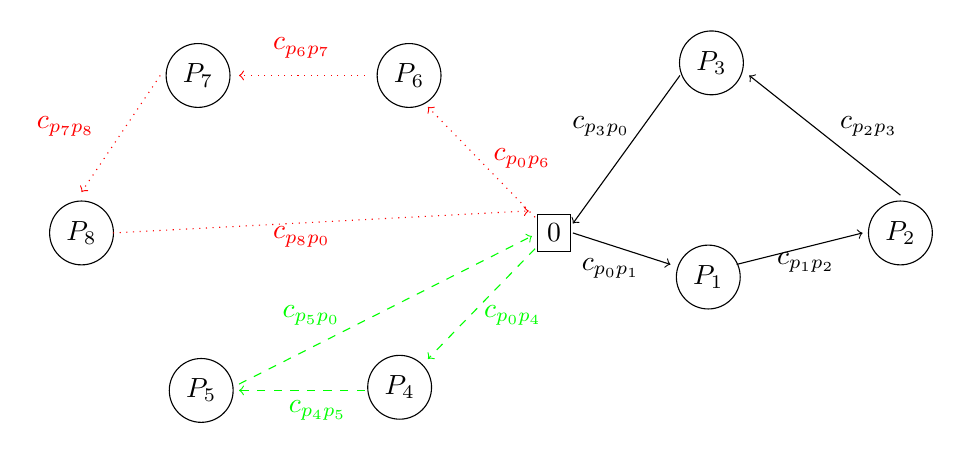
\begin{tikzpicture}[scale=0.4]
	%ponto central
	\draw node[draw] at (0, 0) {$0$};

	%rora 1
   \draw[->, black] (1.8, -0.5) node[below] {$c_{p_0p_1}$} (0.6, 0) -- (3.7, -1.0);
   \draw node[draw, circle] at (4.9, -1.4) {$P_1$};

   \draw[->, black]  (8, -0.3) node[below] {$c_{p_1p_2}$}  (5.8, -1) -- (9.8, 0);
   \draw node[draw, circle] at (11, 0) {$P_2$};

   \draw[->, black] (10, 4) node[below] {$c_{p_2p_3}$} (11, 1.2) -- (6.2, 5);
   \draw node[draw, circle] at (5, 5.4) {$P_3$};
   
   \draw[->, black] (1.5, 4) node[below] {$c_{p_3p_0}$} (4, 5) -- (0.6, 0.3);

	%rota 2
   \draw[->, dashed, green] (-1.3, -2) node[below] {$c_{p_0p_4}$} (-0.6, -0.5) -- (-4, -4);
   \draw node[draw, circle] at (-4.9, -4.9) {$P_4$};
   
   \draw[->, dashed, , green] (-7.5, -5) node[below] {$c_{p_4p_5}$} (-6, -5) -- (-10, -5);
   \draw node[draw, circle] at (-11.2, -5) {$P_5$};
   
   \draw[->, dashed, green] (-7.7, -2) node[below] {$c_{p_5p_0}$} (-10, -4.8) -- (-0.7, -0.1);
   
   %rota 3
   \draw[->, dotted, red] (-1, 3) node[below] {$c_{p_0p_6}$} (-0.6, 0.5) -- (-4, 4);
   \draw node[draw, circle] at (-4.6, 5) {$P_6$};
   
   \draw[->, dotted, red] (-8, 6.5) node[below] {$c_{p_6p_7}$} (-6, 5) -- (-10, 5);
   \draw node[draw, circle] at (-11.3, 5) {$P_7$};
   
   \draw[->, dotted, red] (-15.5, 4) node[below] {$c_{p_7p_8}$} (-12.5, 5) -- (-15, 1.3);
   \draw node[draw, circle] at (-15, 0) {$P_8$};
   
   \draw[->, dotted, red] (-8, 0.5) node[below] {$c_{p_8p_0}$} (-14, 0) -- (-0.8, 0.7);

   );
\end{tikzpicture}
\end{center}
\caption{Exemplo de rotas elaboradas para dois veículos do \ac{SAD} 
\\ \textbf{\footnotesize Fonte: Autoria Própria (2018)}}
\label{grafo1}
\end{figure}


Além das métricas do \ac{PERE} básico, este problema possui diversas métricas que podem ser satisfeitas individualmente ou em conjunto.
A seguir são descritas algumas métricas utilizadas para solucionar o \ac{PERE} de forma a alcançar os devidos objetivos.

\subsection{Equilíbrio de Carga Horária}

Um dos desafios do \ac{PERE} é organizar as visitas que devem ser realizadas por cada enfermeira, de forma que a quantidade de horas trabalhadas não exceda a carga horária máxima estabelecida pela legislação trabalhista e a carga de trabalho seja igualmente distribuída.

Sejam $P_{max}$ e $P_{min}$ os limites superiores e inferiores, respectivamente, das cargas horárias de trabalho de uma enfermeira. O balanceamento de carga horária de trabalho é definido em \citeonline{bachouch:2010} pela seguinte função objetivo: 

\begin{center}
$Min~P_{max} - P_{min}$
\end{center}


Foram apresentados por \citeonline{trabelsi:2012} e \citeonline{bachouch:2010}  modelos de \ac{PLI} tendo como objetivo minimizar discrepância da carga horária de trabalho das enfermeiras, sendo considerados cenários com no máximo três enfermeiras por \citeonline{trabelsi:2012} e com no máximo cinco enfermeiras envolvidas por \citeonline{bachouch:2010}. 
\citeonline{Decerle:2016}  atribuíram um custo a cada hora de trabalho e buscaram minimizar o somatório das horas trabalhadas por cada uma das as enfermeiras, também utilizando um modelo de \ac{PLI}. 
Já \citeonline{cheng:98} elaboraram um modelo de \ac{PLI} com o objetivo de minimizar a quantidade de horas extras de trabalho das enfermeiras. Os mesmos autores propuseram uma heurística gulosa construtiva e obtiveram soluções ótimas para diversas instâncias do problema, sendo consideradas no máximo quatro enfermeiras. 

Foi utilizado o método \textit{Branch‐and-Price‐and‐Cut} para resolver problemas de \acl{PLI} por \citeonline{trautsamwieser:2014}. O modelo proposto pelos autores tem como objetivo minimizar o tempo total trabalhado das enfermeiras. Com esta abordagem foram obtidas soluções ótimas para instâncias em cenários com no máximo duas enfermeiras.  

Foi utilizado por \citeonline{mutingi:2013} uma meta-heurística enxame de partículas para reduzir a diferença entre a carga horária de cada enfermeira pelo valor médio da carga horária de todas as enfermeiras. A técnica proposta foi avaliada utilizando instâncias com até 15 enfermeiras, porém não foi apresentada uma discussão profunda dos resultados obtidos. 

Por fim, \citeonline{luna:2013} buscaram minimizar simultaneamente o número de enfermeiras envolvidas no planejamento e a carga horária total diária. Para isso foi utilizado um algoritmo evolucionário paralelizado, sendo capaz de resolver instâncias com até 32 enfermeiras e mais de 10000 serviços prestados, no entanto os autores não apresentam um estudo da optimalidade das soluções obtidas.

\subsection{Maximização de Satisfação}

Uma forma de tornar o atendimento do \ac{SAD} mais agradável é buscar atender, quando possível, as preferências dos pacientes e das enfermeiras. No contexto do \ac{PERE} estas preferências são tratadas como restrições flexíveis, ou seja, que podem ser violadas caso necessário, porém é desejável que sejam satisfeitas.

Em \citeonline{Bertels:2006} foram definidas as seguintes métricas para determinar as preferências dos pacientes: 

\begin{itemize}
\item Escolher a melhor janela de tempo para receber o atendimento;
\item Escolher o grupo de enfermeiras com as quais deseja ser atendido;
\item Ser atendido sempre pela mesma enfermeira;
\end{itemize}
e das enfermeiras: 
\begin{itemize}
\item Escolher um dos dias da semana para tirar folga;
\item Escolher entre os finais de semana, qual se encaixa melhor em sua organização de trabalho;
\item Trocar de paciente, caso exista alguma dificuldade relacionada a um determinado atendimento.
\end{itemize}


Buscando satisfazer as preferências, das enfermeiras e dos paciente de forma a não prejudicar a qualidade do serviço prestado, \citeonline{Bertels:2006} elaboraram um modelo baseado em Programação por Restrições, tendo como objetivo maximizar a satisfação das enfermeiras, levando em consideração a preferência dos clientes pelas enfermeiras e vice-versa. \citeonline{Bierwirth:2013} e \citeonline{tricoire:2016} propuseram uma abordagem matemática baseada em \ac{PLI} para o \ac{PERE} com o objetivo de maximizar a satisfação dos pacientes.

Em seus experimentos, foi utilizado por \citeonline{Bertels:2006} 120 instâncias sintéticas, contendo entre 20 e 50 enfermeiras, considerando carga horária diária de até nove horas, com o número de pacientes atendidos variando entre 80 e 200 que fazem de 200 a 600 solicitações por dia. A duração de cada atendimento varia entre 6 e 72 minutos e os locais foram escolhidos aleatoriamente, utilizando distâncias euclidianas.
Os resultados foram obtidos em no máximo 232 segundos, com a utilização de instâncias com 50 enfermeiras, 200 pacientes e 600 serviços.

Além de maximizar a satisfação dos clientes \citeonline{Bierwirth:2013} objetivaram minimizar o atraso no atendimento aos pacientes, a distância total percorrida pela equipe e fornecer uma alocação de pacientes de forma a não sobrecarregar uma parte da equipe.

Testes computacionais foram gerados por \citeonline{Bierwirth:2013}  a partir de sete conjuntos de instâncias aleatórias, contendo em cada conjunto, de 10 a 300 pacientes localizados aleatoriamente em uma área quadrada de 100x100 sem levar em consideração a unidade de medida e de 3 a 40 enfermeiras, considerando 6 tipos de serviços, com janela de tempo de 120 minutos, com o tempo limite 10 horas para a execução de cada instância. 
Como resultados, pôde ser observado que pequenas instâncias retornaram resultados ótimos em 20 segundos, enquanto instâncias com mais de 25 pacientes e 5 enfermeiras não conseguiram alcançar bons resultados dentro do tempo estabelecido, sendo necessários o uso de heurísticas mais poderosas.

Além de maximizar a satisfação dos pacientes e enfermeiras, \citeonline{tricoire:2016} também tiveram como objetivo minimizar a distância percorrida pelas enfermeiras, para isso, os autores realizaram experimentos computacionais, a partir de dois conjuntos de instâncias para a execução dos experimentos computacionais. 
O primeiro conjunto contém 30 instâncias de tamanho pequeno, com 20 a 25 serviços e o segundo conjunto é composto por instâncias reais, contendo entre 50 e 300 serviços. 
Para cada instância a carga horária máxima e mínima de trabalho das enfermeiras foi definida entre 8 e 10 horas ou entre 4 e 6 horas, respectivamente, prestando seis tipos de serviços.
O estudo das distâncias percorridas foi gerado a partir da ferramenta OpenStreetMap e dividido em quatro tipos de instâncias, levando em consideração o meio de transporte utilizado pelas enfermeiras (carro ou transporte público) e os experimentos computacionais foram executados no tempo limite de dois dias. Também foram encontrados por \citeonline{tricoire:2016} boas soluções para instâncias de tamanho pequeno, sendo necessário a elaboração de meta heurísticas para elaborar uma solução eficiente para instâncias reais. 

\subsection{Minimização de distâncias}

O estudo da redução das distâncias percorridas pelas enfermeiras do \ac{SAD} tem importância relevante, como foi mencionado por \citeonline{holm:2014}, a extensão do caminho a ser percorrido pelas enfermeiras para atender os pacientes influencia no desgaste sofrido por elas, e consequentemente na qualidade do serviço a ser oferecido, de forma que se um itinerário possui longas distâncias entre as residências dos pacientes, a capacidade de trabalho dessas enfermeiras é afetado.

Motivados pela realidade das empresas de Atenção Domiciliar, \citeonline{tozlu:2016} elaboraram a primeira abordagem do Problema de Roteamento de Veículo da Equipe de Assistência Médica Domiciliar, do inglês, \textit{Crew Constraintes Home Care Routing Problem with Time Window}.
Visando reduzir a distância percorrida pelas enfermeiras em um dia de trabalho, a minimização de distância do \ac{PERE} foi determinada por \citeonline{tozlu:2016} pela seguinte função objetivo:  

\begin{center}
$Min \sum D_{ij}x_{ij}$
\end{center}

Sendo $x_{ij}$ uma variável de decisão que indica que existe um caminho entre $i$ e $j$.

Com o objetivo de reduzir a distância percorrida pelas enfermeiras do \ac{PERE}, foi apresentado um modelo de  \ac{PLI} por \citeonline{Kergosien:2009}, \citeonline{goos:2015}, \cite{Decerle:2016} e \citeonline{tozlu:2016}, enquanto \citeonline{urli:2014} elaboraram de um modelo baseado em Programação por restrições e \citeonline{drake:2007} produziram uma solução utilizando Enxame de Partículas. 

Além do modelo matemático, também foi apresentado por \citeonline{tozlu:2016} um método de Busca por Vizinhança Variável (VNS), do inglês \textit{Variable Neighborhood Search}. 
Em sua abordagem, os autores dividiram a equipe em dois grupos: um grupo de enfermeiras e um grupo de cuidadores e separou os pacientes em três grupos: pacientes que necessitavam de enfermeiras, pacientes que necessitavam de cuidadores e pacientes que necessitavam tando de enfermeiras quanto de cuidadores.
Os veículos utilizados são identificados como tipo 1, tipo 2 e tipo 3.
O objetivo do problema é determinar a rota percorrida e o tipo de veículo que deve atender cada paciente de forma a minimizar a distância percorrida.

Os testes foram realizados por \citeonline{tozlu:2016} a partir de 192 instâncias baseadas nas rotas elaboradas por Solomon para o \ac{PRVJT} com 25 pacientes, encontrando bons resultados para soluções com 175 instâncias dentro do limite de tempo de duas horas. Para o restante das instâncias foi utilizado o melhor resultado retornado.

\citeonline{Kergosien:2009} associaram o \ac{PERE} ao \ac{PRVJT} com algumas restrições relacionadas ao tempo de trabalho e ao atendimento das enfermeiras, também foi notado pelos autores que alguns profissionais não podem prestar serviço simultaneamente, por exemplo: uma enfermeira e um fisioterapeuta. Enquanto alguns serviços necessitam de mais de um profissional, por exemplo: uma enfermeira e um médico. 

Os testes computacionais foram realizados por \citeonline{Kergosien:2009} a partir de 200 instâncias geradas aleatoriamente contendo entre 1 e 3 habilidades e com 20, 30 e 40 serviços com duração entre 10 minutos e uma hora, possuindo a janela de tempo entre meia hora e três horas. Os locais para atendimento foram calculados em espaços euclidianos, em uma área de 100x100. 

O tempo dedicado os testes foi restrito a 10 minutos. Nesse tempo os autores verificaram que a qualidade das soluções está diretamente ligado ao número de habilidades, já que o número de soluções encontradas aumenta quando o número de habilidades diminui.

Os profissionais do \ac{PERE} foram classificados por \citeonline{Decerle:2016} entre licenciados e não licenciados. Os profissionais licenciados oferecem serviços médicos, como administração de remédios, tratamentos de saúde enfermagem, já os profissionais não licenciados oferecem serviços de apoio domiciliar, tais como auxílio nas tarefas domésticas e de higiene.

Experimentos computacionais foram elaborados por \citeonline{Decerle:2016} a partir dos dados obtidos em duas empresas de Assistência Domiciliar não identificadas pelos autores. Nessas empresas, as enfermeiras trabalham entre $6:45 am$ até $7:30 pm$, a janela de tempo de visita tem a duração máxima de uma hora. Os profissionais licenciados possuem um custo de 50 euros por hora e os profissionais não licenciados possuem o custo de 30 euros por hora.

Os experimentos foram executados no tempo máximo de uma hora. Como resultados, pode ser observado que o método de \ac{PLI} foi eficiente em retornar soluções para pequenas instâncias, sendo necessário a utilização de meta heurísticas para tratar de instâncias maiores nesse tempo.

Além do método de Programação por Restrições, também foi elaborada por \citeonline{urli:2014} a técnica Branch-and-Bound, e a meta-heurística LNS, do inglês \textit{Large Neighborhood search}, que visa explorar uma grande vizinhança de soluções. A formulação do problema e os resultados baseados em restrições do mundo real, foram cedidas pela empresa especializada em soluções de software para escalonamento de problemas, chamada EasyStaff.

Para a realização dos testes computacionais, foram gerados aleatoriamente por \citeonline{urli:2014} 18 grupos com 30 instâncias cada, totalizando 540 instâncias, em um local de 40 $Km^{2}$, localizada no centro de Udine, Itália, diferenciadas pelo horizonte de planejamento. 
A partir dos resultados estudados, os autores chegaram a conclusão que o LNS supera a Programação por Restrições quando se trata de atividades não atribuídas, por outro lado, a técnica de Programação por Restrições é superior a LNS quando se trata de reduzir a distância total de deslocamento.


Foram apresentados por \citeonline{drake:2007} dois experimentos computacionais utilizando instâncias reais com 9 clientes, que recebem cuidados de enfermeiras e cuidadores, no período de uma semana.
O primeiro experimento analisa o desempenho da técnica apresentada com diferentes configurações de parâmetros em diferentes instâncias de problemas usando o design de experimentos de Taguchi, um tipo de experimento que ao administrar fatores de controle minimizam os ruídos, no qual os autores utilizaram como fator de controle as distâncias viajadas e buscaram minimizar o tamanho da equipe de atendimento e maximizar a satisfação dos clientes. 
O segundo experimento consistiu em comparar as soluções obtidas manualmente pelo governo do Reino Unido, com as soluções obtidas pelos autores.

Foi realizado por \citeonline{goos:2015} um estudo de caso, tendo com o objetivo de maximizar a qualidade do serviço e minimizar a distância percorrida pelas enfermeiras da organização, no qual Os experimentos foram executados a partir de instâncias reais obtidas na empresa estudada, contendo no total 478 pacientes,  que são atendidos por 115 enfermeiras, que prestam serviços médicos e de assistência domiciliar.
 
\subsection{Outras Métricas}

Além da métrica de equilíbrio de carga horária, maximização de satisfação e minimização de distância, alguns pesquisadores utilizaram outras métricas de pesquisa para solucionar algumas questões do \ac{PERE}, tais como problemas envolvendo minimização do tamanho da equipe. Para solucionar o problema de minimização do tamanho da equipe, foram elaboradas soluções baseadas em \acl{PLI}, por \citeonline{calvo:2013}. \citeonline{rasmussenm:2012} foi elaboraram uma técnica baseada em \textit{Branch and Price} para resolver o problema de Programação Inteira Linear, \citeonline{nguyen:2016} utilizaram Algoritmos Genéticos e \citeonline{cattafi:2012} utilizaram a técnica de Programação por Restrições, para encontrar uma boa solução para o \ac{PERE}.

Foi introduzido por \citeonline{nguyen:2016} um modelo integrado do \ac{PERE} no qual características realistas como incerteza na disponibilidade do enfermeiro, restrições legais de horário e de trabalho são levadas em consideração.
Para solucionar o problema, \citeonline{nguyen:2016} lidaram com quatro problemas de otimização: \textit{rostering, assignment, routing, and scheduling} de forma sequencial e iterativa. 
Como resultados foi observado que o algoritmo proposto funciona melhor com a estratégia de substituir soluções ao acaso, é eficiente para a solução de grandes instâncias e fornece uma solução confiável contra a incerteza na disponibilidade de enfermeiros para o planejamento semanal e pode ser uma ferramenta para avaliar o \textit{trade-off} entre a robustez e o custo operacional de uma solução.

Um estudo de caso foi realizado por \citeonline{cattafi:2012} com o objetivo de minimizar a carga horária máxima de trabalho e minimizar a quantidade de enfermeiras diferentes que visitam o mesmo paciente. Testes computacionais foram realizados com 15 enfermeiras, que atendem a 3323 requisições de 458 pacientes em um mês de trabalho, sendo que cada requisição e tem a duração variando entre 5 a 60 minutos. 
Como resultado os autores concluíram que a técnica de Programação Lógica é uma tecnologia economicamente acessível para melhorar as condições de trabalho e a qualidade dos serviços.

Em \citeonline{calvo:2013}, os autores se empenharam em minimizar o número de enfermeiras, utilizando Programação Linear Inteira para pequenas instâncias e uma meta heurística para os testes com médias instâncias. 
Os experimentos computacionais foram realizados com o auxílio de 190 instâncias, propostas por \citeonline{Kergosien:2009}, contendo 30 serviços, prestado por 7 a 9 enfermeiras possuindo até 3 habilidades. 

Por fim, \citeonline{rasmussenm:2012} realizaram um estudo com o objetivo minimizar o número de visitas não cobertas e os custos totais da viagem, além de maximizar a preferência de visitas de cuidadores.
Os testes computacionais foram feitos com 4 instâncias reais obtidas no hospital municipal dinamarquês e algumas instâncias sintéticas baseadas nas instâncias reais, além de 60 instâncias geradas pelos autores.



